\chapter{Implementation}
\label{chap:implementation}

In the previous chapter we saw how EzQL provides some new features and
abstractions that allow it to stand on a higher-level compared to
traditional event processing languages. In general, this is a good
thing, because the language becomes easier and more expressive at the
hands of the developer. However, the higher the language is, the
farther it is from machine-level, which also means harder to
compile. This is even more true in a domain-specific language such as
EzQL with its uncommon execution model. In order to guarantee that
``high-level'' does not become ``stratospherically high-level'', a proof
of concept implementation has been written. The goal of this chapter
is to explain the pragmatics and describe the main challenges that had
to be overcome in order to create this prototype.

\section{The pipeline}

EzQL, the event processing engine, is an evaluator that analyzes the
code in multiple stages, from its textual form to a runtime
representation, simpler to execute, conceptually similar to query
plans. The following sections discuss these phases in more detail.

\begin{figure} \centering
  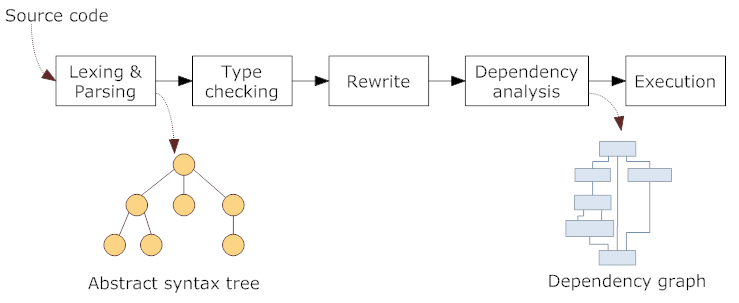
\includegraphics[width=0.8\textwidth]{phases.png}
  \caption{An overview of the analysis process.}
  \label{fig:phases}
\end{figure}

\subsection{Lexing and parsing}
\label{sub:lexing-parsing}

Lexing and parsing are two standard procedures in programming language
pragmatics. These two phases are responsible for what is usually
called ``syntactic analysis''. Ever since the first compilers were
written, syntactic analysis received a great deal of attention. Along
the years, this research produced a set of tools -- Lex and Yacc
\cite{lex-yacc} --, that has greatly simplified this task, to the
point where programming language researchers don't give it much
attention anymore, preferring to address theoretic foundations and
semantic concerns instead. As expected, EzQL uses these tools, which
means the biggest challenge in this phase was to guarantee that the
grammar was unambiguous, which is not much of a challenge these days.

\subsection{Type checking}
\label{sub:type-checking}

Type-checking -- including type-inference --, is implemented through
the well-known Damas-Milner algorithm\footnote{Out of curiosity,
  Lu\'{i}s Damas is a Portuguese researcher at the University of
  Porto.} \cite{damas-milner}. This algorithm works in two phases:
constraint collection and unification.

The first phase consists in performing a pass over the abstract syntax
tree produced by the parser and collecting a set of typing
constraints. For example, the following listing taken from the
previous chapter,

\begin{lstlisting}
  def printEvents (s, fn) =
      when ev in s -> print (fn(ev))
\end{lstlisting}

produces the following constraints:

\begin{enumerate}
\item \verb=printEvents= is a function that receives two parameters
  with initial types \verb='s= for the type of \verb=s= and \verb='f=
  for the type of \verb=fn=, and returns some other unknown type
  \verb='r=;
\item While it analyzes the \verb=when=, the type checker infers that
  the type of \verb=s= -- \verb='s= -- must be \verb=stream<'a>= for
  some event type \verb='a=. Also, the type of \verb=ev= must be
  \verb='a=;
\item Since \verb=fn= is called with \verb=ev=, \verb=fn= must be a
  function that receives an \verb='a= and returns some other type
  \verb='t=;
\item \verb=print= is a primitive function that receives anything and
  returns \verb=unit=, which means nothing. \verb=unit= plays a
  similar role to \verb=void= in C-like languages;
\item The return type of the entire \verb=when= expression must be the
  same as the return type of \verb=print=;
\item Finally, the return type of the entire function -- \verb='r=,
  must be the same as the return type of the \verb=when= expression,
  because there is nothing following the \verb=when=.
\end{enumerate}

Note that, at this point, the algorithm does not try to solve these
constraints, no matter how trivial the solution seems to be. This
happens only in the second phase, where the unification algorithm
tries to find consistent types for all terms. For the constraints
above, the algorithm finds out that:

\begin{itemize}
\item \verb=s= is of type \verb=stream<'a>=. Since there are no
  constraints regarding the type of the events in \verb=s=, the
  algorithm settles on the generic \verb='a= type, which essentially
  means ``accept any stream'';
\item \verb=fn= is a function that receives an \verb='a= and returns a
  \verb='r=. The return type has not been constrained because
  \verb=print= is a polymorphic function that accepts anything;
\item Finally, since \verb=print= returns \verb=unit=, so does
  \verb=when= and so does \verb=printEvents=. Thus, \verb=printEvents=
  accepts a \verb=stream<'a>=, a function from \verb='a= to \verb='r=
  and returns \verb=unit=.
\end{itemize}

Note that there is an implicit constraint between \verb=s= and
\verb=fn=, because they both reference the type \verb='a=. This means
that the type checker will guarantee that all calls to
\verb=printEvents= use consistent arguments. For example, the
following snippet would be refused:

\begin{lstlisting}
  stocks = stream of { timestamp:int, symbol:string, price:float }

  def not (b) =
    if b then false else true

  printEvents (stocks, not)
\end{lstlisting}

For this particular application, the type checker will try to replace
\verb='a= with the type of the events in the stream --
\verb={ timestamp:int, symbol:string, price:float }= which is not
consistent with the type of \verb=not=, which expects a simple
\verb=bool=.

\subsection{Rewriting phase}
\label{sub:rewriting}

Rewriting transforms the abstract syntax tree in order to lighten the
work that needs to be done by the remaining phases. In particular, it
takes most of the syntactic sugar that was added to make the language
more user-friendly -- but contains no semantic value whatsoever --,
and replaces it with more primitive constructs. It is interesting to
analyze a few transformations, to see how the runtime relies on these
primitives to implement higher-level features:

\begin{description}
\item[Function definitions] are transformed into simple variable
  definitions with anonymous function values:

  \begin{lstlisting}
    def not (b) =
      if b then false else true
  \end{lstlisting}

  is transformed into:

  \begin{lstlisting}
    not = fun b -> if b then false else true
  \end{lstlisting}

\item[Entity definitions] including associations, are transformed into
  \verb=group by= expressions, as alluded in section
  \ref{sec:entities};
\item[SQL-syntax] is transformed into an alternative ``method call''
  syntax more familiar to OOP programmers that we have not presented
  yet. For example, the following listing taken from section
  \ref{sec:streams-windows}

  \begin{lstlisting}
    from ev in stocks
    where ev.symbol == "ACME"
    select { price_x2 = ev.price * 2 }
  \end{lstlisting}

  is equivalent to:

  \begin{lstlisting}
    stocks
      .where  (fun ev -> ev.symbol == "ACME")
      .select (fun ev -> { price_x2 = ev.price * 2 })
  \end{lstlisting}

  While it seems less user-friendly, this syntax is more explicit and
  shows operators for what they really are: methods of the
  \verb=stream= class. In the case of \verb=where= and \verb=select=
  it also shows that the predicate and the projector are actually
  anonymous functions passed as parameters to these methods. This is
  interesting because if the developer is, somehow, allowed to
  implement these methods in EzQL, he will be able to create new
  operators without modifying the syntax of the language. More on this
  in chapter \ref{chap:eval}.

\end{description}

\subsection{Dependency analysis}
\label{sub:dataflow}

EzQL programs are composed by a number of definitions, or queries. The
results of these queries may be stored in variables and used by other
queries. As we have seen in chapter \ref{chap:ezql}, when a variable
is updated, its changes are propagated downward, so that other queries
that depend on it may be immediately updated too. This process
continues until there are no more changes left to spread. Furthermore,
it is not enough to simply propagate these changes -- we must do it in
the correct order too. To see why, suppose you have the following
definitions:

\begin{lstlisting}
  acmePrice = acmeStocks.last().price # current ACME's price
  xptoPrice = xptoStocks.last().price # current XPTO's price
  sumPrices = acmePrice + xptoPrice
\end{lstlisting}

Here, \verb=acmeStocks= contains only price reports from the financial
market related to ACME while \verb=xptoStocks= contains
XPTO's. Suppose a new event arrives into \verb=acmeStocks=: first
\verb=acmePrice= should be updated, and then \verb=sumPrices=. Now
suppose that, at the same time, new events arrive on both the
\verb=acmeStocks= and \verb=xptoStocks= streams: the system must
update both \verb=acmePrice= and \verb=xptoPrice= before it updates
\verb=sumPrices=.

To propagate values the right way, the engine performs some dependency
analysis over the code, which results in a dependency graph. This
graph also records the operators that should be used for each step of
the query, a characteristic it shares with query plans. An example of
this analysis is shown next, where the code below gives origin to the
graph in figure \ref{fig:graph1}.

\begin{lstlisting}
  stocks = stream of { timestamp:int, symbol:string, price:float }

  # For each company, calculates the ratio between the current price
  # and the maximum price of all companies.
  ratioOverMax =
    from ev in stocks
    group by :symbol into events
    select
      let currPrice = events.last().price
      let maxPriceOverall = stocks.max(:price)
      currPrice / maxPriceOverall
\end{lstlisting}

\begin{figure}[t]
  \centering
  \subfloat[Main graph]{\label{fig:graph1}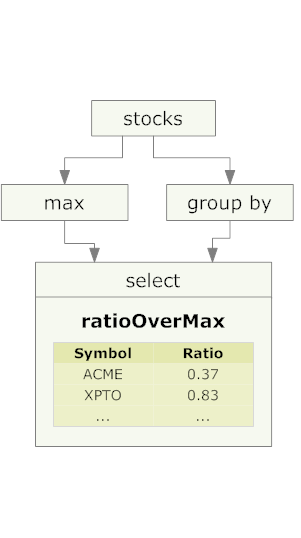
\includegraphics[width=0.25\textwidth]{ratioMax.png}}
  \subfloat[Main graph with select's inner graph]{\label{fig:graph2}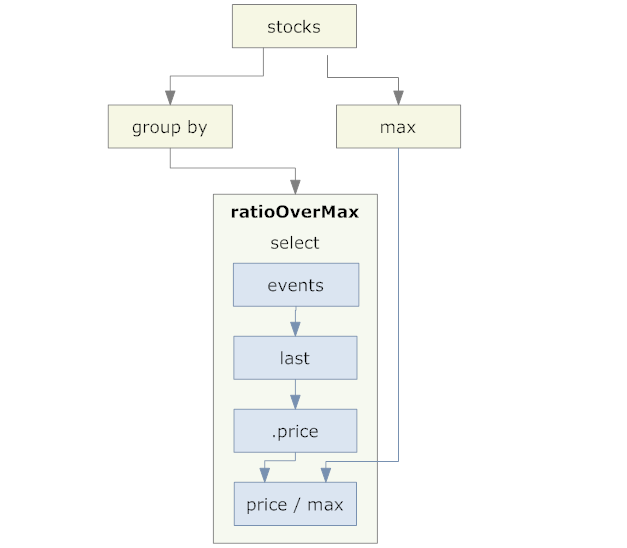
\includegraphics[width=0.5\textwidth]{ratioMax-expanded.png}}
  \caption{Dependency graph for \tt{ratioOverMax}}
\end{figure}


This example takes, once again, the \verb=stocks= stream and
calculates, for each company, the ratio between its current price and
the maximum price overall (not necessarily from the same company). In
the resulting graph we can see that the calculation of
\verb=maxPriceOverall= -- through the \verb=max= operator -- has been
taken out of the \verb=select=, which is allowed because it doesn't
depend on \verb=events=. On the other hand, the maximum becomes a
parent of \verb=select=, which makes sense: if the maximum changes, we
want \verb=ratioOverMax= to be immediately re-evaluated.

This raises an interesting question: to re-calculate the ratio of all
companies we will need the current price of each one of them. In some
cases however, this price may have been set by an event that arrived
minutes or even hours ago. Thus, in order to execute this query, the
system must store the current price of each company. How does it know
which values to keep?

The answer is that \verb=select= contains an inner graph that tells it
which operators are needed to execute the projection and which values
must be kept, as shown in figure \ref{fig:graph2}. This graph starts
with \verb=events=, which represents a stream with the events for each
group, and flows down to the node that is responsible for calculating
the final result (labeled \verb=price/max=). Note that the maximum
price is defined in the outer graph, but referenced by the inner
graph. This hierarchical structure may be extended for many more
levels. The following example illustrates this:

\begin{lstlisting}
  wereThere =
    from room in Room.all
    select (from product in Product.all
            where (product.room == room)[5 min].any?()).count()
\end{lstlisting}

\begin{figure}[t]
  \centering
  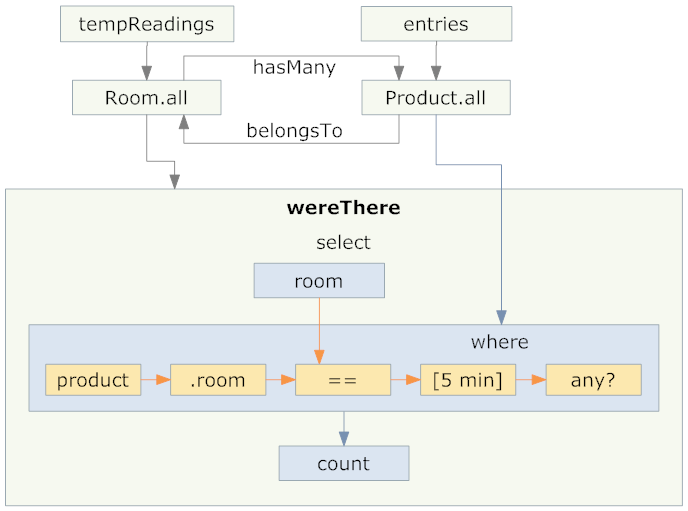
\includegraphics[width=0.6\textwidth]{wereThere.png}
  \caption{Dependency graph for \tt{wereThere}}
  \label{fig:graph-wereThere}
\end{figure}

This creates a dictionary that contains, for each \verb=Room=, the
number of products that were there at any moment during the last 5
minutes. The entire graph is shown in figure
\ref{fig:graph-wereThere}. As we can see, \verb=where= also has an
internal graph that is necessary to keep the 5 minutes window and the
result of the \verb=.any?()= aggregator. The interesting part is that
this internal graph references \verb=room=, which is part of the
\verb=select='s graph, which also references \verb=Product.all=,
defined in the outer scope. Whenever a product switches rooms,
\verb=Product.all= will propagate that change down to the
\verb=where=, the predicate will be updated and so will the
\verb=count()=. This culminates with the update of the \verb=select=,
whose result will be kept in \verb=wereThere=. Besides changes to
products, the five minutes windows, buried inside graphs of graphs as
they are, may ignite the update process, at any moment, due to the
expiration of some event. Moreover, if two of these things happen at
the same time, we will have two updates in parallel, which the system
must handle carefully in order to avoid messing up the results. All
this, however, happens during execution, which is the topic of the
next section.

\subsection{Execution}
\label{sub:execution}

After the dependency analysis is complete, the engine uses the graph
to create a network with the operators that will compute the results
during execution. Much like graph nodes may contain inner graphs, this
network's operators may also contain inner-networks. For example, the
\verb=where= operator uses its inner-graph to create an inner-network
for each entry that is added to the dictionary. This inner-network is
used to keep historic data necessary to calculate the result of the
predicate. This means the network is dynamic: when a new entry is
added to the dictionary, a sub-network is created just for it. Figure
\ref{fig:network} illustrates this.

\begin{figure} \centering
  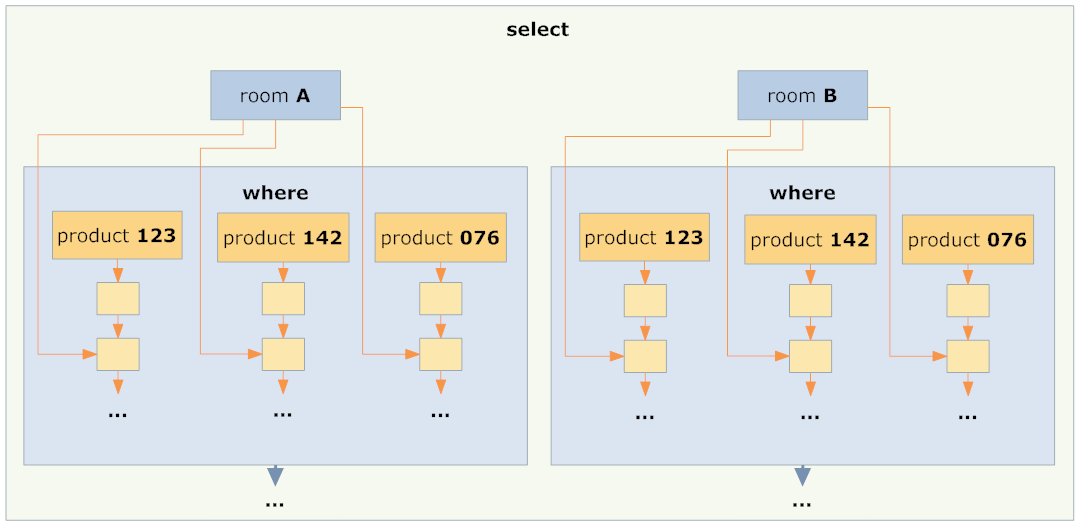
\includegraphics[width=0.8\textwidth]{network.png}
  \caption{During execution, the select and where operators for
    dictionaries replicate their sub-networks for each entry in the
    dictionary they are applied to. In this example, there are two
    rooms -- A and B -- and three products -- 123, 142 and 076 -- in
    the system.}
  \label{fig:network}
\end{figure}


Given that in EzQL queries run forever, the operators don't pass
complete results to each other. Instead, they communicate by sending
incremental changes. For example, when an event is added to a window,
the update signal that is propagated contains only the event, not the
entire window. Similarly when a new entry is added to a dictionary,
the dictionary propagates a change saying that the value at the given
key was updated. Moreover, these changes may be recursive. For
example, if the values of the dictionary are windows (which is allowed
in EzQL), the changes propagated by the dictionary contain the changes
propagated by the windows, and so on.

There are a total of 34 operators implemented in this prototype. They
can be classified into:

\begin{description}
\item[Stream and window operators], including the operators that
  represents a stream and a window, \verb=select= and \verb=where= for
  streams and windows, \verb=groupby=, \verb=when=, \verb=changes=,
  \verb=last= and \verb=sort=;
\item[Dictionary operators] corresponding to \verb=select= and
  \verb=where= for dictionaries, as well as \verb=values=;
\item[Aggregators], including: \verb=count=, \verb=sum=, \verb=avg=,
  \verb=min=, \verb=max=, \verb=any?=, \verb=all?=, \verb=howLong=;
\item[Other operators] a category that includes operators to represent
  function calls, records, indexers into dictionaries, field
  projectors out of records and an operator that implements an
  interpreter and is capable of executing some simple expressions.
\end{description}

The freedom EzQL provides allows for some unexpected combinations of
these operators. Creating dictionaries of other dictionaries, opening
timed windows inside function definitions, storing streams inside
record fields, are some rather surprising combinations that EzQL does
not forbid. Coordinating all these operators and testing some of the
infinite ways one can join them together, consumed a major part of
this work. The single task of coming up with an architecture flexible
enough to support our requirements -- the need to create and destroy
operators during runtime, operators that may depend on other operators
situated in different networks, the handling of simultaneous events
and expirations -- took some thought to mature. Still, that is not the
end of the story.

\section{Complications on a scheme}
\label{sub:complications}

\subsection{Round and around}

The graph that is created by the dependency analysis cannot contain
cycles, otherwise the changes propagation algorithm may not
terminate. Fortunately, cyclic dependencies are forbidden by design: a
definition cannot reference other definitions declared below. There
is, however, an exception to this rule: the
\verb=belongsTo=/\verb=hasMany= combo may need to refer to an
undeclared entity. For example, in

\begin{lstlisting}
  entity Product =
    createFrom (entries, :productId)
    belongsTo :room

  entity Room =
    createFrom (tempReadings, :roomId)
    hasMany :products
\end{lstlisting}

\verb=belongsTo= refers to the \verb=Room= entity, which has not yet
been declared. This has consequences on two stages of the code
analysis: type checking and dependency analysis. The type checker will
fail because it can't find the type of the \verb=room= field that
\verb=belongsTo= adds to the \verb=Product= entity. The dependency
analysis algorithm, on the other hand, will fail because it can't find
the \verb=Room.all= dictionary which is a dependency of
\verb=Product.all=.

Our solution consists in performing a normal pass over the code. If an
undeclared reference is found, though, an exception is thrown and the
algorithm records the field that caused the problem and the unknown
reference. In the example above, the \verb=room= field created by the
\verb=belongsTo= would cause an exception, because the entity
\verb=Room= had not yet been declared. The algorithm would then
proceed as if the \verb=room= field did not exist. When \verb=Room=
had been analyzed, the algorithm would check if there were any pending
operations that depend on it and would find that \verb=Product= needed
to be re-checked, which it would do right away. This operation may
take a few iterations to complete if both entities depend on each
other in intricate ways (for example, if \verb=Room= needs the
\verb=room= field of any of its \verb=products=).

\subsection{Filter doesn't actually filter}

In section \ref{sub:associations} we alluded to a problem related to
filtered dictionaries and historic data used in predicates or
projections over them. This happened while discussing the following
example:

\begin{lstlisting}
  wereInRoomB =
    from p in Room.all["A"].products
    where (p.roomId == "B")[5 min].any?()
\end{lstlisting}

The \verb=where= predicate asks for the results of the condition
\verb!p.roomId == "B"! over the last 5 minutes, for all products that
are in room A. However, the system must keep this information for all
products -- not just for the ones in room A --, because, as far as the
system is concerned, a product may switch to room A at any moment, and
when it does, the 5 minutes history must be readily available.

The prototype copes with this situation by keeping data for the hidden
entries inside dictionaries. Thus, dictionaries contain both hidden
and visible entries and handle them the same way. When an hidden entry
is updated, its changes are propagated as usual, except they are
tagged as being hidden, so that other operators may keep them
invisible to the outside. For example, if the application tries to
index a hidden entry with \verb=wereInRoomB[<hiddenProductId>]=, the
result will be \verb=null=.


\section{Testing and validation}
\label{sec:testing}

In order to test the prototype and to verify it gives correct answers,
we developed a small testing library. This library tests the engine
using a black-box approach: it sends events into the input streams and
checks if the monitored operators react accordingly. Furthermore, if
an unexpected events occurs, a warning will be emitted.

Currently, the prototype comes with a test-suite encompassing about
140 test cases and more than 900 assertions.
